\documentclass[twoside,11pt]{article}
\usepackage[slovene]{babel}
\usepackage[utf8]{inputenc}
\usepackage{graphicx}
\usepackage[frame]{matrika}
\usepackage{mathtools}
\usepackage{epstopdf}
\usepackage{units}

\usepackage{amsmath} % enačbe
\usepackage[thinc]{esdiff} % za odvode
\usepackage[colorlinks=false]{hyperref} % za linke
\usepackage{float} % za fiksiranje figur
%\usepackage[sorting=none,doi=false,isbn=false,eprint=false,url=false]{biblatex}
\usepackage{csquotes}
% Po potrebi se lahk dodajo drugi standardni paketi, ki ne spreminjajo izgleda dokumenta

%\addbibresource{viri.bib}
\newcommand{\dif}[1]{\,{\rm d}#1}

\begin{document}

\MAT{2}{11}{2024}
\naslov{Fotonika kvantnih pik}

\avtor{Vito Levstik}

\institucija{Fakulteta za matematiko in fiziko \\ Univerza v Ljubljani}

\klasifikacija{~} 
\izvlecek{Kvantne pike so polprevodniški nanokristali, v katerih so energijski nivoji zaradi majhne velikosti kvantizirani. Posledično so energije
izsevanih fotonov natančno določene. Področje kvantnih pik je precej aktualno, kar dokazuje podeljena Nobelova nagrada za kemijo leta 2023. Ta članek služi
kot pregled vsebin, za katero je bila podeljena. Članek najprej predstavi zgodovino raziskovanja področja in nato teoretični
model izsevanja fotonov vse od enostavnega modela potencialne jame do raznih popravkov osnovnega modela. Na koncu predstavi še postopek sinteze kvantnih pik in nekatera področja, kjer so kvantne pike uporabne.}
\title{Photonics of quantum dots}
\abstract{Quantum dots are semiconducting nanocrystals in which energy levels are quantized because of their small size. As a consequence the energies of emitted
photons are exactly determined. The field of quantum dots is popular lately, as evidenced by Nobel prize for chemistry in 2023. This article serves
as an overview of the topics for which the prize was awarded. The article first describes the history of reasearch of the field and
then the theoretical model of photon emission, starting with particle in a box model and additional corrections to it. Finally, it describes the process of quantum dot synthesis and some areas where quantum dots are used.}

\glava\baselineskip=14.5pt

\smallskip

\section{Uvod}
Leta 2023 je bila Nobelova nagrada za kemijo podeljena Moungi G. Bawendiju, Louisu E. Brusu in Alekseyu Yekimovu za odkritje in sintezo kvantnih pik v 80-ih letih prejšnjega stoletja \cite{nobel}. 

Že stoletja znajo steklarji izdelovati barvna stekla, tako da dodajo primesi različnih kovin ter spreminjajo temperaturo staljenega stekla \cite{doi:10.1021/acsnano.1c01399}. 
Aleksey Yekimov je z uporabo žarkov X določil velikosti kristalov primesi in ugotovil, da se s spreminjanem velikosti kristalov spreminja barva stekla. Temu opazovanju je takoj pripisal kvantnomehansko naravo \cite{nobel}.
Neodvisno od Yekimova je Louis Brus prav tako prišel do istega spoznanja, le da je on opazoval nanodelce v tekočinah \cite{doi:10.1021/acsnano.1c01399}. Ti nanodelci so kasneje dobili ime kvantne pike.
Po odkritju je formuliral teoretični model, ki je pojasnil energijo izsevanih fotonov, ki nastanejo ob rekombinaciji elektrona in vrzeli, za različne velikosti nanodelcev \cite{nobel}.
Vendar so se kvantne pike, ki jih je proizvedel Brus, znatno razlikovale v velikosti. Moungi Bawendi je s procesom koloidne sinteze drastično izboljšal produkcijo kvantnih pik, tako v kvaliteti, kot tudi v količini \cite{nobel}.

Od takrat so kvantne pike postale že praktično uporabne. Med drugim se uporabljajo v zaslonih \cite{https://doi.org/10.1002/anie.202004857, doi:10.1021/acs.chemrev.2c00695}, biosenzorjih \cite{doi:10.1126/science.281.5385.2013}, sončnih celicah \cite{doi:10.1021/jz400052e}, laserjih \cite{laser} in drugod. 
Celoten trg kvantnih pik je bil leta $2021$ ocenjen na $4$ milijarde dolarjev in naj bi do leta $2026$ zrasel na kar $8.6$ milijard \cite{market}. Ideje o uporabi kvantnih pik so prisotne tudi v kvantnem računalništvu \cite{PhysRevA.57.120}.

V prvem delu tega članka si pogledamo teoretični opis, kako pride do generacije fotonov in kako je njihova energija povezana
z lastnostmi kvantnih pik, v drugem delu pa predstavimo proces sinteze kvantnih pik in nekaj področij, kjer so te uporabne.
 
\section{Teoretični opis}
\label{sec:teoretični_opis}
Kvantne pike so $0$--dimenzionalni polprevodniški nanokristali, kjer so kvantni efekti tisti, ki določajo njihove karakteristike. Pri tem se število $0$ nanaša na število prostih dimezij kristala. Z absorpcijo svetlobe se elektron iz valenčnega pasa vzbudi v
prevodni pas in za seboj pusti pozitivno vrzel v valenčnem pasu. To se zgodi samo, če je energija absorbiranega fotona večja ali enaka razliki energije med prevodnim in valenčnim pasom.
Elektron v višjih nivojih v prevodnem pasu se lahko preko relaksacijskih procesov spusti v najnižje stanje tik ob robu prevodnega pasu. Čez čas se tak elektron rekombinira z vrzeljo iz valenčnega pasu, pri čemer se izseva
foton, katerega energija je točno določena zaradi kvantiziranih energijskih nivojev v valenčnem in prevodnem pasu \cite{basic}. Nobelov nagrajenec Louis Brus je pokazal, da so
kvantni pojavi v kvantnih pikah odvisni od velikosti samih nanokristalov. Formuliral je model, ki pojasni energijsko odvisnost izsevanih fotonov
od velikosti kvantnih pik.

\subsection{Brusov model}
Da je Brus pojasnil obnašanje elektrona in vrzeli v sistemu, je naredil sledeče predpostavke in približke \cite{doi:10.1021/ed079p1094}:
\begin{enumerate}
   \item Nanokristal je sferičen s polmerom $R$.
   \item Notranjost kristala je uniformna in v njej ni nobenih točkastih nabojev, razen vzbujenega elektrona in vrzeli.
   \item Potencialna energija zunaj nanokristala je neskončna, zato elektron in vrzel vedno najdemo v notranjosti nanokristala.
\end{enumerate}

\subsubsection{Točkast naboj}
Najprej poglejmo obnašanje enega nabitega delca v kristalu, za katerega veljajo predpostavke Brusovega modela. Dobljeni rezultati nam bodo pomagali v nadaljevanju, ko bomo obravavali par elektron-vrzel v kvantnih pikah.

Zanimajo nas lastne funkcije in lastne energije delca. Hamiltonijan za prost točkast naboj je

\begin{equation}
   H = -\frac{\hbar^2}{2m_{ef}}\nabla^2 + V(r) \; ; \quad V(r) = \begin{cases}
                                                   0,  & r < R \\
                                                   \infty,  & r > R
                                                   \end{cases},
\end{equation}
kjer je $m_{ef}$ efektivna masa točkastega naboja in $r$ razdalja od središča nanokristala.
Ker je potencial odvisen samo od radija, imamo torej problem centralnega potenciala, zato se lahko $H$ razstavi na radialni in kotni del

\begin{equation}
   H = -\frac{\hbar^2}{2m_{ef}} \left( \frac{1}{r^2} \frac{\partial}{\partial r} r^2 \frac{\partial}{\partial r}\right) + \frac{L^2}{2m_{ef}r^2} + V(r), 
\end{equation}
kjer je $L^2$ vrtilna količina \cite{kvantna_ramšak}.

Rešujemo stacionarno Schrödingerjevo enačbo. Primeren nastavek za lastno funkcijo je produktna funkcija $\varPsi(r, \vartheta, \varphi) = \psi_l(r) Y_l^m(\vartheta, \varphi)$, kjer je $Y_l^m$ sferični harmonik
in $\psi_l(r)$ radialni del funkcije. 
Upoštevamo, da je potencial znotraj kvantne pike $0$ in da so lastne vrednosti operatorja vrtilne količine določene z $L^2 Y_l^m = l(l+1)\hbar^2 Y_l^m$.
Spomnimo, da je kvantno število $m$ omejeno z $|m| \le l$. Radialni del Schrödingerjeve enačbe se tako preoblikuje v
\begin{equation}
   \label{eq:radialna_SE}
   \frac{\partial^2 \psi}{\partial r^2} + \frac{2}{r} \frac{\partial \psi}{\partial r} + \left(k^2 - \frac{l(l+1)}{r^2}\right)\psi = 0,
\end{equation}
kjer je $k^2 = 2mE/\hbar^2$.

Rešitev enačbe (\ref{eq:radialna_SE}) je linearna kombinacija sferične Besselove funkcije prve in druge vrste $\psi_l(r) = A_l j_l(kr) + B_l y_l(kr)$, pri čemer sta funkciji definirani kot

\begin{equation}
   j_l(x) = \sqrt{\frac{\pi}{2x}}J_{l+1/2}(x), \quad y_l(x) = \sqrt{\frac{\pi}{2x}}Y_{l+1/2}(x),
\end{equation}
kjer sta $J_l(x)$ in $Y_l(x)$ Besselovi funkciji prve in druge vrste \cite{abramowitz1965handbook}. Ker $y_l(x)$ divergira, ko gre $x$ proti $0$, mora biti $B_l = 0$ za vsak $l$.
Hkrati mora biti $\psi(R) = 0$, kar tvori robni pogoj $j_l(kR) = 0$. Naj bo $\xi_{n,l} = kR$ $n$-ta ničla funkcije $j_l$. Tako je lastna valovna funkcija točkastega naboja enaka

\begin{equation}
   \varPsi(r, \vartheta, \varphi) = A_l j_l\left(\xi_{n,l} \frac{r}{R}\right) Y_l^m(\vartheta, \varphi),
\end{equation}
kateri ustreza lastna energija
\begin{equation}
   E = \frac{\hbar^2}{2m_{ef}R^2}\xi_{n,l}^2.
\end{equation}

Lastna stanja so torej opisana s tremi kvantnimi števili $n,l,m$. Opazimo, da lastna energija ni odvisna od števila $m$, torej imamo degenerirane energijske nivoje. Popravimo oznako za lastne funkcije
v $\varPsi_{n,l,m}(r, \vartheta, \varphi)$ in oznako za lastne energije v $E_{n,l}$.

Dodatno si poglejmo primer, ko je $l = 0$ in posledično $m=0$. Tedaj je $j_0(x)=\sin(x) / x$ \cite{abramowitz1965handbook}, torej so ničle $\xi_{n,0} = n\pi$, za $n = 1,2,3,...$
Po normalizaciji in ob upoštevanju, da je $Y_0^0(\vartheta, \varphi) = 1/(2\sqrt{\pi})$, je lastna valovna funkcija odvisna samo od radija $r$
\begin{equation}
   \label{eq:valovna_en_delec}
   \varPsi_{n,0,0}(r) = \frac{1}{r\sqrt{2\pi R}} \sin \left(\frac{n\pi}{R} r\right). 
\end{equation}
Ustrezna lastna energija je
\begin{equation}
   \label{eq:energija_en_delec}
   E_{n,0} = \frac{\hbar^2 \pi^2}{2mR^2}n^2.
\end{equation}

\subsubsection{Eksciton}
\label{sec:eksciton}
Z absorpcijo fotona se elektron preseli v prevodni pas, pri čemer za seboj pusti pozitivno vrzel. Nastane par elektron-vrzel oziroma eksciton. To pomeni, da 
sta sočasno v kristalu dva nabita delca. Ker so kvantne pike polprevodniški nanokristali in glede na 2. predpostavko Brusovega modela, ki pravi, da sta edina točkasta naboja v notranjosti kvantne pike le vzbujena elektron in vrzel,
to pomeni, da je elektron (vrzel) edini nabiti delec v prevodnem (valenčnem) pasu. Iz tega sledi, da je bil pred absorpcijo valenčni pas zapolnjen, prevodni pas pa prazen.
Hamiltonijan v notranjosti kvantne pike v tem primeru postane

\begin{equation}
   \label{eq:H_interakija}
   H = -\frac{\hbar^2}{2m_e}\nabla_e^2 -\frac{\hbar^2}{2m_v}\nabla_v^2 + V(\vec{r}_e, \vec{r}_v), 
\end{equation}
kjer $V(\vec{r}_e, \vec{r}_v)$ označuje potencial zaradi medsebojne interakcije. Vektorja $\vec{r}_e$ in $\vec{r}_v$ označuje\-ta položaja elektrona in vrzeli v kvantni piki, merjena od središča kvantne pike, masi $m_e$ in $m_v$ pa sta efektivni masi elektrona in vrzeli. Privzeli bomo, da je medsebojen potencial
samo posledica Coulombove interakcije, in sicer
\begin{equation}
   V(\vec{r}_e, \vec{r}_v) = -\frac{e^2}{4\pi \varepsilon \varepsilon_0 |\vec{r}_e - \vec{r}_v|},
\end{equation}
kjer je $e$ naboj elektrona in vrzeli in $\varepsilon$ dielektrična konstanta za notranjost kvantne pike.

Hamiltonijan v enačbi (\ref{eq:H_interakija}) ni enostavno rešljiv zaradi medsebojne interakcije. Analitični približek za najnižjo energijo
ekscitona je \cite{doi:10.1021/j100403a003}
\begin{equation}
   \label{eq:E_exciton}
   E_{ex} = \frac{\hbar^2 \pi^2}{2R^2}\left(\frac{1}{m_e}+\frac{1}{m_v}\right) - \frac{1.8e^2}{4\pi \varepsilon \varepsilon_0 R}.
\end{equation}

Do tega rezultata lahko pridemo na sledeč način. Najprej zanemarimo medsebojno Coulombsko interakcijo. V tem primeru je valovna
funkcija sistema določena s produktom lastnih funkcij za posamezen delec \cite{glenn_rowe}
\begin{equation}
   \Psi(r_e, r_v) = \varPsi_e(r_e)\varPsi_v(r_v),
\end{equation}
kjer je funkcija $\varPsi(r)$ podana z enačbo (\ref{eq:valovna_en_delec}). Skupna energija sistema je zato kar vsota lastnih energij
\begin{equation}
   E_{ex} = \frac{\hbar^2 \pi^2}{2R^2}\left(\frac{1}{m_e}+\frac{1}{m_v}\right).
\end{equation}
Ker se zanimamo za energijo najnižjega stanja, je kvantno število $n$ za elektron in vrzel enako $1$. Coulombski potencial upoštevamo tako,
da za razdaljo $d=|\vec{r}_e - \vec{r}_v|$ uporabimo povprečno razdaljo med nabojema, ki znaša $d = R/1.8$ \cite{doi:10.1021/ed079p1094}.
Tako dobimo nek efektiven konstanten potencial, ki ga samo prištejemo k energiji in dobimo željen rezultat -- enačbo (\ref{eq:E_exciton}).

Energija, ki jo nosi izsevan foton ob rekombinaciji elektrona in vrzeli, je enaka
\begin{equation}
   \label{eq:Brus}
   E = E_g + \frac{\hbar^2 \pi^2}{2R^2}\left(\frac{1}{m_e}+\frac{1}{m_v}\right) - \frac{1.8e^2}{4\pi \varepsilon \varepsilon_0 R},
\end{equation}
kjer je $E_g$ energijska reža med valenčnim in prevodnim pasom snovi, iz katere je narejena kvantna pika \cite{doi:10.1021/ed079p1094}.
Enačba (\ref{eq:Brus}) je znana kot \textit{Brusova enačba}. 

Potrebna je še razlaga, od kod pride člen $E_g$. Po absorpciji fotona je elektron v 
prevodnem pasu, zato je njegova energija enaka energiji roba prevodnega pasu $E_c$, ki ji prištejemo kvantizirano energijo (enačba (\ref{eq:energija_en_delec})) elektrona z efektivno maso $m_e$ \cite{doi:10.1021/j100403a003}
\begin{equation}
   E_e = E_c + \frac{\hbar^2 \pi^2}{2m_eR^2}.
\end{equation}

\begin{figure}[H]
   \begin{center}
       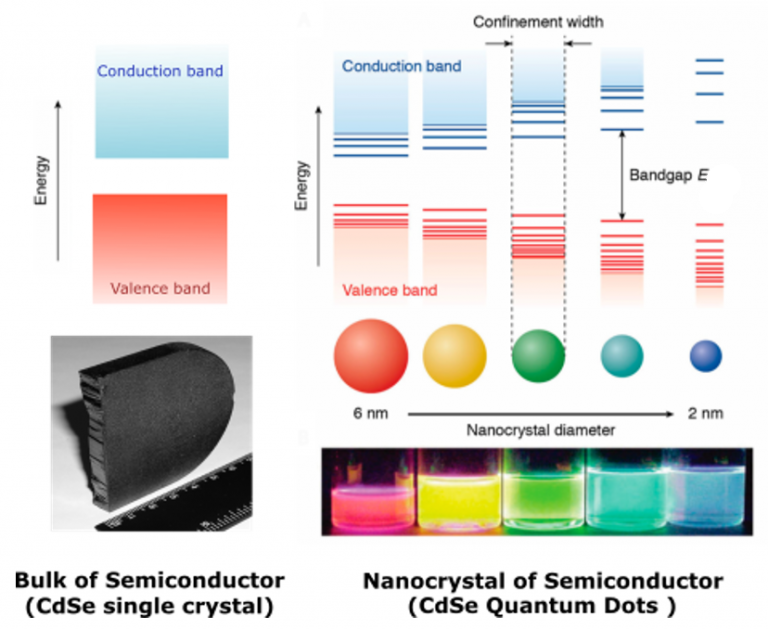
\includegraphics[width=13cm]{figures/band_gap.png}
       \caption{Shematska predstava odvisnosti energijske razlike od velikosti kvantnih pik in primerjava s 3D polprevodnikom za kvantne pike iz kadmijevega selenida (CdSe). Z rdečo barvo so označeni energijski nivoji v valenčnem pasu, z modro pa so označeni energijski nivoji v prevodnem pasu. V kvantnih pikah so energijski nivoji kvantizirani, medtem ko so v 3D polprevodniku zvezni. Vir: \cite{basic}.}
       \label{fig:band_gap_in_QD_and_bulk}
   \end{center}
\end{figure}

S podobnim razmislekom lahko pridemo do energije vrzeli
\begin{equation}
   E_{vr} = E_v - \frac{\hbar^2 \pi^2}{2m_vR^2},
\end{equation}
kjer je $E_v$ energija roba valenčnega pasu in $m_v$ efektivna masa vrzeli. Foton se izseva ob rekombinaciji elektrona in vrzeli, torej je njegova energija
\begin{equation}
   \label{eq:E_foton}
   E = E_e - E_{vr} = E_g + \frac{\hbar^2 \pi^2}{2R^2}\left(\frac{1}{m_e}+\frac{1}{m_v}\right),
\end{equation}
pri čemer smo upoštevali definicijo energijske reže $E_g = E_c - E_v$. V tem postopku nismo upoštevali prispevka k energiji zaradi Coulombskega potenciala, ki bi se efektivno razdelil med elektronom in vrzeljo.

Alternativno lahko do člena $E_g$ pridemo z razmislekom, da pri naši
računici za energijo ekscitona (enačba (\ref{eq:E_exciton})) nismo upoštevali dejstva, da moramo najprej tvoriti eksciton, tako da dvignemo elektron iz valenčnega
v prevodni pas, pri čemer potrebujemo $E_g$ energije.

Slika \ref{fig:band_gap_in_QD_and_bulk} shematsko prikazuje kako se energijski nivoji v kvantnih pikah spreminjajo s spreminjanjem velikosti kvantnih pik. Energijska razlika $E$ med osnovnima nivojema v valenčnem in
v prevodnem pasu je opisana z \textit{Brusovo enačbo}.

\subsection{Natančnejši opis}
V tem poglavju obravnavamo različne popravke osnovnega Brusovega modela kvantnih pik.

\subsubsection{Prispevek polarizacije}
V enačbi (\ref{eq:H_interakija}) smo za potencial upoštevali samo Coulombsko interakcijo med elektronom in vrzeljo. V resnici obstaja še prispevek potenciala zaradi polarizacije. Točkast naboj
v notranjosti nanokristala le-tega polarizira in s tem dodatno vpliva na drug naboj. Izkaže se, da je energija zaradi tega efekta v primerjavi z Coulombovo in kinetično energijo
precej manjša \cite{doi:10.1021/ed079p1094}, zato polarizacije do sedaj nismo obravnavali. Polarizacijski člen je podan z
\begin{equation}
   V(\vec{r}_e, \vec{r}_v) = \frac{e^2}{2} \sum_{k=1}^{\infty} \alpha_k \frac{|\vec{r}_e|^{2k}+|\vec{r}_v|^{2k}}{R^{2k+1}},
\end{equation}
kjer je
\begin{equation}
   \alpha_k = \frac{(\eta-1)(k+1)}{4\pi \varepsilon \varepsilon_0 (\eta k + k + 1)}, \quad \eta=\frac{\varepsilon}{\varepsilon_{zun}}
\end{equation}
in $\varepsilon_{zun}$ označuje dielektrično konstanto zunanjega medija, ki obdaja nanokristal. Izkaže se, da je popravek k energiji ekscitona zaradi polarizacije enak \cite{doi:10.1021/ed079p1094}
\begin{equation}
   E_{pol} = \frac{e^2(\eta - 1)}{2\pi R^2 \varepsilon \varepsilon_0} \int_{r=0}^{R} \sin^2 \left(\frac{\pi r}{R}\right) \sum_{k=1}^{\infty} \frac{k+1}{(\eta + 1)k + 1} \left(\frac{r}{R}\right)^{2k} \dif{r}.
\end{equation}

\begin{figure}
   \begin{center}
       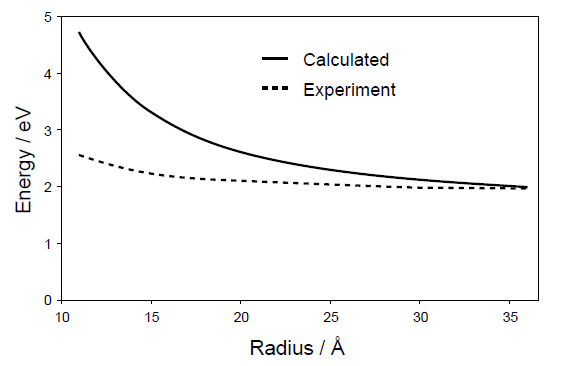
\includegraphics[width=11cm]{figures/energija_funkcija_radija.png}
       \caption{Energija izsevanih fotonov kot funkcija radija za kvantno piko iz CdSe. Polna črta označuje teoretično napoved, kjer je upoštevan prispevek Coulombskega potenciala in prispevek polarizacije, medtem ko črtkana črta označuje eksperimentalo izmerjeno energijo. Vir: \cite{doi:10.1021/ed079p1094}.}
       \label{fig:energija_funkcija_radija}
   \end{center}
\end{figure}

Slika \ref{fig:energija_funkcija_radija} prikazuje energijo izsevanih fotonov kot funkcijo radija kvantne pike, narejene iz kadmijevega selenida, pri čemer je upoštevan tudi popravek zaradi polarizacije. Pri majhnih radijih je razkorak med teoretično napovedjo
in eksperimentalo vrednostjo velik, medtem ko je za večje radije ujemanje boljše.

\subsubsection{Končen potencial}
Do zdaj smo upoštevali Brusov model, ki je privzel neskončen potencial zunaj kvantne pike. Neskončen potencial fizikalno ni mogoč, zato bi natančnejša obravnava 
zahtevala, da je potencial zunaj kvantne pike končen.

Naj bo potencial zunaj nanokristala $V$. Z enačbo $V = \hbar^2 \nu^2 / 2mR^2$ uvedemo brezdimenzijski parameter $\nu$, kjer je $R$ radij nanokristala in $m$ efektivna masa delca. Energija delca $E$ bo zagotovo manjša od $V$, torej
jo lahko zapišemo kot
\begin{equation}
   \label{eq:E_finite_barrier}
   E = V - \frac{\hbar^2 \beta^2}{2mR^2} = \frac{\hbar^2 \alpha^2}{2mR^2},
\end{equation}
s čimer smo povezali parametre $\alpha^2 + \beta^2 = \nu^2$. Ker je ta obravnava še vedno problem centralnega potenciala, je valovna funkcija še vedno
produkt radialnega dela ter sferičnega harmonika $\varPsi(r, \vartheta, \varphi) = \psi_l(r) Y_l^m(\vartheta, \varphi)$. Izkaže se, da je rešitev radialnega dela valovne funkcije podana z \cite{LEYRONAS2001631}
\begin{equation}
   \begin{split}
      \psi_l(r < R) &= A\sqrt{\frac{R}{r}}J_{l+1/2}\left(\alpha \frac{r}{R}\right), \\
      \psi_l(r > R) &= A\sqrt{\frac{R}{r}}\frac{J_{l+1/2}(\alpha)}{K_{l+1/2}(\beta)}  K_{l+1/2}\left(\beta \frac{r}{R}\right),
   \end{split}
\end{equation} 
kjer je $J_l(x)$ Besselova funkcija prve vrste, $K_l(x)$ modificirana Besselova funkcija druge vrste in $A$ normalizacijska konstanta. Zanima nas najnižji energijski nivo, torej $l=0$. V tem primeru
se izraza za valovni funkciji poenostavita, saj je $J_{1/2}(x)=(2/\pi x)^{1/2} \sin x$ in $K_{1/2}(x)=(\pi/2x)^{1/2}e^{-x}$:
\begin{equation}
   \label{eq:valovna_finite}
   \begin{split}
      \psi_0(r < R) &= A\sqrt{\frac{2}{\pi \alpha}} \frac{R}{r} \sin \left(\alpha \frac{r}{R}\right) \\
      \psi_0(r > R) &= A\sqrt{\frac{2}{\pi \alpha}} \frac{\sin \alpha}{e^{-\beta}} \frac{R}{r} e^{-\beta \frac{r}{R}} = A\sin \alpha \sqrt{\frac{2}{\pi \alpha}} \frac{R}{r} e^{-\beta \left(\frac{r}{R} - 1\right)}.
   \end{split}
\end{equation}

Zaradi pogoja zveznosti odvoda valovne funkcije pri $r=R$ to vodi v transcendentno enačbo $\alpha / \tan \alpha = - \beta$ oziroma $\nu = \alpha / |\sin \alpha|$ \cite{LEYRONAS2001631}.

Z aproksimacijo transcendentne enačbe
\begin{equation}
   \alpha(\nu) \approx \frac{\pi \nu}{1 + \nu + \frac{(\pi/2-1)^2}{\nu-1}},
\end{equation}  
in upoštevanjem enačbe (\ref{eq:E_finite_barrier}) dobimo končno rešitev za energijo izsevanega fotona v primeru končnega potenciala \cite{Ferreira_2017}:
\begin{equation}
   \label{eq:E_finite_barrier_final}
   E = E_g + \frac{\hbar^2}{2m_eR^2}\left[\frac{\pi \nu_e}{1 + \nu_e + \frac{(\pi/2-1)^2}{\nu_e-1}}\right]^2 + \frac{\hbar^2}{2m_vR^2}\left[\frac{\pi \nu_v}{1 + \nu_v + \frac{(\pi/2-1)^2}{\nu_v-1}}\right]^2.
\end{equation} 
Pri tem sta parametra $\nu_e$ in $\nu_v$ povezana s potencialom kot $V = \hbar^2 \nu_i / 2m_iR^2$. 

Preverimo še, da v limitnem primeru dobimo enako rešitev kot v poglavju \ref{sec:eksciton} \,. Neskončnemu potencialu ustreza $\nu = \infty$. Posledično je $\alpha = \pi$ in $\beta = \infty$.
Izraz za energijo (\ref{eq:E_finite_barrier_final}) se poenostavi v izraz (\ref{eq:E_foton}). Prav tako se valovna funkcija, ki opisuje nabit delec (enačba (\ref{eq:valovna_finite})), poenostavi v
\begin{equation}
   \begin{split}
      \psi_0(r < R) &\propto \frac{1}{r} \sin \left(\pi \frac{r}{R}\right),\\
      \psi_0(r > R) &= 0,
   \end{split}
\end{equation}
kar ustreza valovni funkciji nabitega delca v neskončnem potencialu. Omenimo, da v tej obravnavi ekscitona v končnem potencialu nismo upoštevali prispevkov zaradi Coulombove interakcije in polarizacije.

\section{Koloidna sinteza}
Kvantne pike se lahko proizvede na več načinov. Pomemben način, ki je hkrati enostaven in zato primeren za masovno proizvodnjo, je
koloidna sinteza. Moungi Bawendi je ravno s to metodo revolucioniral proces proizvodnje, za kar je z Alekseyem Yekimovom in z Louisom Brusom letos dobil Nobelovo nagrado za kemijo.

Koloidna sinteza kvantnih pik se začne z vbrizganjem materiala, iz katerega bodo nastale kvantne pike, v vroče topilo z visokim vreliščem, pri čemer
se zgodi takojšnja piroliza materiala. Hitro povišanje koncentracije reagenta povzroči hitro supersaturacijo in nukleacijo kvantnih pik. Zaradi vbrizganja temperatura pade,
zaradi česar se rast kvantnih pik ustavi. S ponovnim segrevanjem na željeno temperaturo se rast počasi nadaljuje. S tem procesom dobimo makroskopske količine
kvantnih pik, ki imajo dobro definirane velikosti ravno zaradi možnosti natančnega kontroliranja temperature \cite{nobel}. Shematski prikaz koloidne sinteze je prikazan na sliki \ref{fig:koloidna_sinteza}.

\begin{figure}[H]
   \begin{center}
       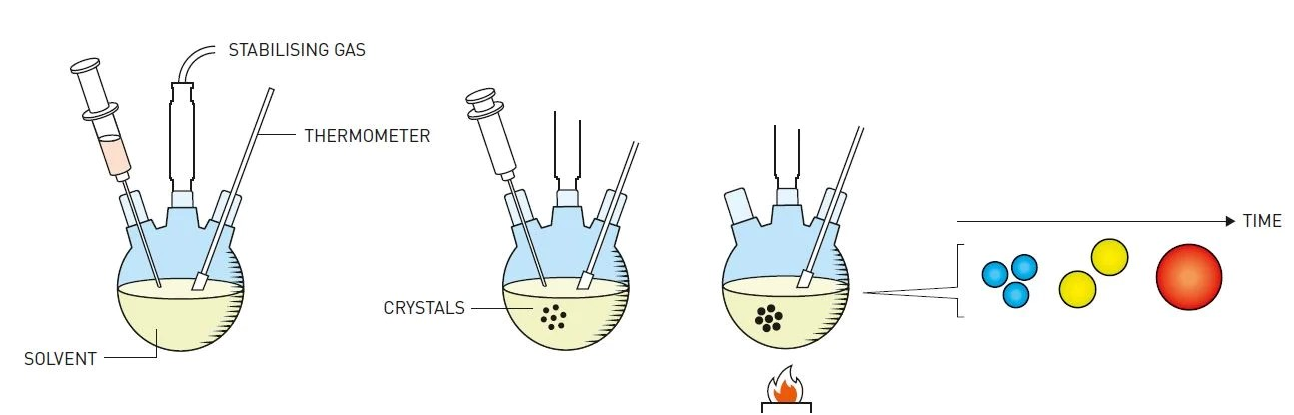
\includegraphics[width=16cm]{figures/koloidna_sinteza.png}
       \caption{Shema procesa koloidne sinteze kvantnih pik. V zaprto posodo, v kateri je vroče topilo, se vbrizga material. Ta se nabere skupaj, s čimer se tvorijo kvantne pike. Z nadaljnim segrevanjem kvantne pike rastejo, torej je njihova velikost odvisna od časa segrevanja. Vir: \cite{nobel2}.}
       \label{fig:koloidna_sinteza}
   \end{center}
\end{figure}

\section{Aplikativnost}
Kvantne pike so predvsem zaradi fino nastavljive energijske reže s spreminjanjem velikosti in materiala ter enostavnosti proizvodnje zelo atraktivne za uporabo v industriji. Uporabljajo se v zaslonih, fotovoltaiki, biosenzorjih, fotodetektorjih in celo v kvantnem računalništvu.
V tem poglavju si bomo ogledali dve najbolj razširjeni področji, kjer se kvantne pike uporabljajo -- zaslone in sončne celice.

\subsection{Zasloni}
V splošnem lahko zaslone s kvantnimi pikami razdelimo v dve skupini: fotoluminiscenčne (foto-emisivne) in elektroluminiscenčne (elektro-emisivne). 
V obeh primerih so kvantne pike tiste, ki izsevajo fotone, vendar je mehanizem izsevanja različen. Grafični prikaz delovanja obeh tipov zaslonov
je prikazan na sliki \ref{fig:zasloni}.

\begin{figure}[H]
   \begin{center}
       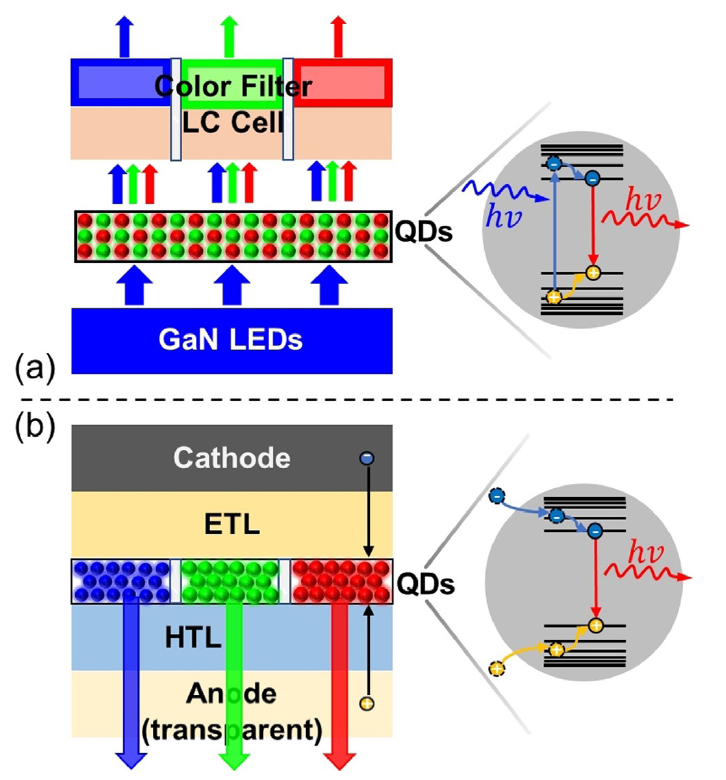
\includegraphics[width=10cm]{figures/zasloni.png}
       \caption{Shematska predstava delovanja enega piksla pri zaslonih tipa (a) QD-LCD in (b) QLED. QD-LCD zasloni delujejo s pomočjo tekočih kristalov (LC Cell), ki vpadno svetlobo, ki delno izvira iz kvantnih pik, bodisi prepusti ali pa ne. V QLED zaslonih pa kvantne pike določenih barv doziramo s pari elektron-vrzel, ki se rekombinirajo in izsevajo foton. Vir: \cite{https://doi.org/10.1002/anie.202004857}.}
       \label{fig:zasloni}
   \end{center}
\end{figure}

\subsubsection{Foto-emisivni zasloni}
Foto-emisivni zasloni so po delovanju podobni tradicionalnim LCD zaslonom, zato so znani pod kratico QD-LCD. V teh zaslonih je anorganski
fosfor v \textit{backlight} mehanizmu, ki pri vzbuditvi osvetljuje piksle z belo svetlobo, zamenjan s širokim spektrom zelenih in rdečih kvantnih pik, ki so osvetljene z modro svetlobo LED diod \cite{https://doi.org/10.1002/anie.202004857}. Način delovanja takšnega zaslona je sledeč: najprej je vsak
piksel osvetljen z modrimi LED diodami (GaN). Del svetlobe se v kvantnih pikah absorbira, le-te pa nato emitirajo nazaj fotone v zeleni in rdeči barvi. Tako
dobimo svetlobo iz modrih, rdečih in zelenih fotonov, ki pade na tradicionalno celico iz tekočega kristala za posamezen pod-piksel, ki vpadno svetlobo bodisi prepusti ali ne. 
Na koncu je prepuščena svetloba barvno filtrirana glede na to, za kateri pod-piksel gre (moder, rdeč, zelen). 

V takšnih zaslonih je energijski izkoristek še vedno precej nizek, saj mora pri konstantni intenziteti svetlobe, ki jo generirajo modre LED diode, barvni filter v 
vsakem pod-pikslu odstraniti približno $2/3$ fotonov \cite{https://doi.org/10.1002/anie.202004857}.

\subsubsection{Elektro-emisivni zasloni}
Elektro-emisivni zasloni so bolje poznani pod kratico QD-LED ali QLED. V teh zaslonih vsak pod-piksel vsebuje le kvantne pike ustrezne barve in neodvisen tranzistor. Samo takrat, ko mora biti pod-piksel prižgan, tranzistor injicira skozi plast transporta elektronov (ETL) in skozi plast transporta vrzeli (HTL) točno določeno
količino parov elektron-vrzel, ki se v kvantnih pikah rekombinirata, pri čemer se izseva foton. Zaradi tega imajo QLED zasloni
izjemno dober barvni kontrast ter bistveno boljšo energijsko učinkovitost v primerjavi z QD-LCD zasloni \cite{https://doi.org/10.1002/anie.202004857}.

\subsection{Sončne celice}
Sončne celice predstavljajo še eno področje, kjer so kvantne pike zelo zanimive za uporabo. Maksimalna termodinamična učinkovitost za pretvorbo iz sončne v električno energijo v enojnem stiku p-n je približno $31\%$, kar je znano kot Shockley-Queisserjeva limita. 
Glavni faktor, ki limitira maksimalno učinkovitost je, da je preostanek energije absorbiranega fotona izgubljen v obliki toplote. Vodilni pristop, kako zmanjšati te izgube, je uporaba večih p-n
stikov z različnimi energijskimi režami. To so t.i. \textit{multi-junction solar cells}. Tako so fotoni z višjimi energijami absorbirani v polprevodnikih z višjo energijsko režo, medtem ko so fotoni z nižjo energijo absorbirani v polprevodnikih z 
nižjo energijsko režo. S takim pristopom, kjer popolnoma zajamemo sončev spekter, je teoretična učinkovitost $66\%$ \cite{NOZIK2002115}.

Sončne celice s kvantnimi pikami uporabljajo kvantne pike kot glavni absorber fotonov. Zaradi njihove nastavljive energijske reže, ki se spreminja z velikostjo, so uporabne v \textit{multi-junction} sončnih celicah,
kjer zamenjajo tradicionalne polprevodnike \cite{sinovoltaics}. Shematska predstava njihove sestave je prikazana na sliki \ref{fig:QD_solar_cell}.
\begin{figure}[H]
   \begin{center}
       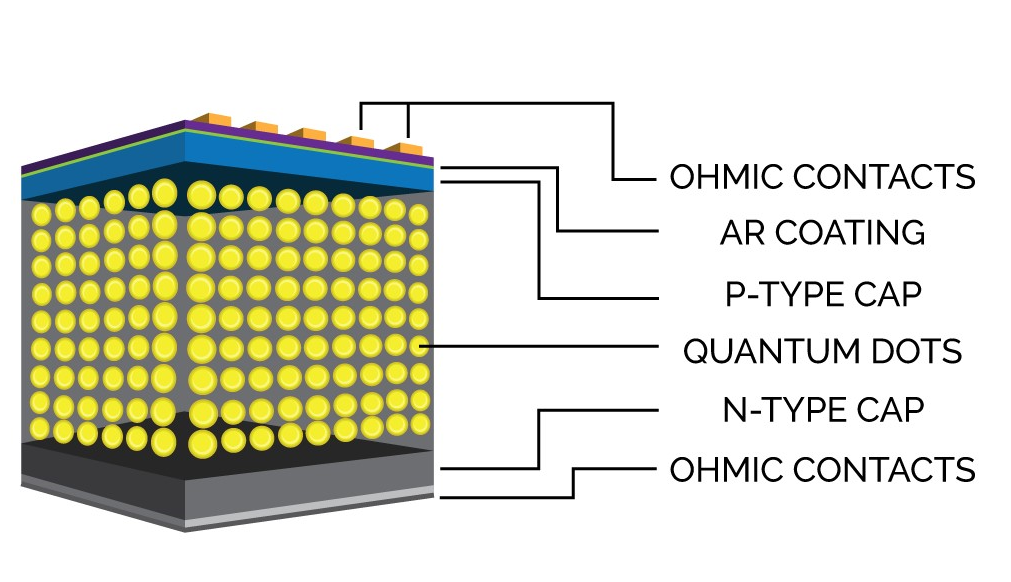
\includegraphics[width=10cm]{figures/QD_solar_cell.png}
       \caption{Shematska sestava sončne celice z uporabo kvantnih pik. Kvantne pike (označene z rumeno barvo) se nahajajo med p-tipom polprevodnika (označen z modro barvo) in n-tipom polprevodnika (označen s sivo barvo) in so glavno območje, kjer se fotoni absorbirajo. Vir: \cite{sinovoltaics}.}
       \label{fig:QD_solar_cell}
   \end{center}
\end{figure}

\section{Zaključek}
Kvantne pike so izjemno aktualno področje, kar dokazuje podeljena Nobelova nagrada leta 2023. Kljub zapleteni geometriji in sestavi kvantnih pik, lahko glavne poteze njihovega obnašanja opišemo s preprostimi kvantnomehanskimi modeli. 
Enostaven in razširjen model je Brusov model, ki pojasni, kako je energija izsevanih fotonov odvisna od velikosti kvantnih pik.
Za natančnejši izračun energij lahko Brusov model izboljšamo z upoštevanjem prispevka polarizacije in z upoštevanjem končnega potenciala. 
Kvantne pike se danes že uporabljajo v zaslonih, saj nudijo boljši energijski izkoristek in boljši barvni kontrast. 
Prav tako uporaba kvantnih pik v sončnih celicah obeta boljšo energijsko učinkovitost.

\bibliographystyle{amsplain_nosort.bst}
\bibliography{viri.bib}

\end{document}
